\chapter{Implementation}
\label{chap:implementation}
\section{Preparations}
\subsection{Setting up a virtual machine}

For all developments within this thesis a virtual machine was used. This makes it easy to reproduce the environment within the labs at the TKRN group as well as having a portable development solution isolated from the rest of the computer's operating system. As the ROS version called \textit{Kinetic} is widely used within the set-ups around the robot, I will also develop the application using this version. This reduces the risk of incompatibility issues during development. ROS \textit{Kinetic} is available as packages for Ubuntu up to version 16.04\cite{ros:install}, which is why we install this version of Ubuntu within a new virtual machine. Enough virtual hard disk space and memory is assigned to the virtual machine (200GB HDD, 8 GB RAM) as well as 4 processing cores. This set-up should be sufficient for all purposes during this thesis. 

If the virtual machine shall run ROS nodes which have to be accessible by ROS nodes outside the machine itself (i.e. the Android tablet running the control application) the network interface of the virtual machine should be configured as a bridged network connection. This lets the network's DHCP (if present) assign the virtual machine its own IP address reachable from the network. However, this was not possible within the university's network, as Oracle VirtualBox was not able to create a working bridged network adapter using the computer's Wi-Fi connection. During development within the lab another computer directly connected to the university network was used to run \textit{roscore}.

\subsection{Setting up ROS}

\subsubsection{Installing ROS}

Setting up ROS \textit{Kinetic} within a fresh Ubuntu 16.04 installation is fairly simple. First, the ROS apt\footnote{Aptitude is the package management system for Debian-based Linux distributions like Ubuntu}-repository has to be added to the packages sources file and the corresponding key has to be added to the key storage to enable downloading the packages. Once this is done, the package \textit{ros-kinetic-desktop-full} can be installed which will download and install all available packages for ROS \textit{Kinetic}.

The commands to install ROS are denoted in Listing \ref{lst:ros:install}. After these commands have been executed in a terminal window ROS is readily installed.

\begin{minipage}{\linewidth}
	\begin{lstlisting}[caption={Commands for installing ROS\cite{ros:install}},label={lst:ros:install}]
	sudo sh -c 'echo "deb http://packages.ros.org/ros/ubuntu $(lsb_release -sc) main" > /etc/apt/sources.list.d/ros-latest.list'
	sudo apt-key adv --keyserver hkp://ha.pool.sks-keyservers.net:80 --recv-key 421C365BD9FF1F717815A3895523BAEEB01FA116
	sudo apt-get update
	sudo apt-get install ros-kinetic-desktop-full
	\end{lstlisting}
\end{minipage}

ROS is by default installed to \textit{/opt/ros/kinetic/}. To make use of all available command line tools provided by ROS it is important to load the file \textit{/opt/ros/kinetic/setup.bash} into the currently open (bash)-command-prompt. This is either temporarily done by issuing

\begin{lstlisting}[caption={Temporarily loading the ROS environment into bash}]
source /opt/ros/kinetic/setup.bash
\end{lstlisting}

or permanently by adding this line to the file \textit{$\sim$/.bashrc} by executing the following command:

\begin{lstlisting}[caption={Permamently installing the ROS environment into bash}]
echo "source /opt/ros/kinetic/setup.bash" >> ~/.bashrc
source ~/.bashrc
\end{lstlisting}

When this is done, ROS is completely set up on the development machine.

\subsubsection[Setting up catkin]{Setting up a catkin workspace\cite{ros:install:catkin}} 

\textit{Catkin\footnote{\url{http://wiki.ros.org/catkin}}} is a build system and workspace management utility provided with ROS. It supports developers to create, develop and build packages for ROS applications. To create a catkin workspace within the current user's home directory, issue the commands from Listing \ref{lst:ros:catkin} after setting up ROS and sourcing the \textit{setup.bash}-file.

\begin{minipage}{\linewidth}
	\begin{lstlisting}[caption={Setting up a catkin workspace},label=lst:ros:catkin]
mkdir -p ~/catkin_ws/src
cd ~/catkin_ws/
catkin_make

source devel/setup.bash
	\end{lstlisting}
\end{minipage}

ROS and catkin are now fully set up and can be used for further development.

\subsection{Installing Android Studio}

Android Studio is used as IDE during development of this thesis and should be installed according to the official documentation\footnote{\url{https://developer.android.com/studio/install.html}}. It is sensible to add the \textit{bin} directory within Android Studio's installation path to the \textit{PATH} environment variable to make Android Studio accessible by just typing \textit{studio.sh} into a terminal window.

After Android Studio was installed successfully, it is important to select and install the correct Android SDK versions as the project will compile with the Android 7 compiler to work with Android 4. To do so, open The SDK Manager (\textit{Tools > Android > SDK Manager}) and select the SDKs according to Figure \ref{fig:android:sdk}. When this is done, Android Studio is set up to develop and compile the application.

\begin{figure}
	\caption{Needed Android SDKs\label{fig:android:sdk}}
	\begin{center}
		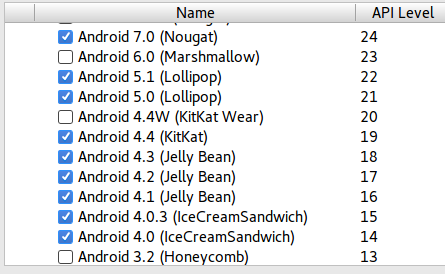
\includegraphics[scale=0.7]{assets/chpt_impl/sdks.PNG}
	\end{center}
\end{figure}

\subsection{Modifying and compiling rosandroid}
\label{impl:compiling_rosandroid}

Since the application developed in this thesis shall work on Android from versions beginning at 4.0.3 we have to modify the rosandroid code on one little detail to make everything work fine. In the created catkin workspace, go to the \textit{src} folder and clone the rosjava and rosandroid repositories there:
\begin{lstlisting}[caption={Cloning the rosandroid and rosjava repositories}]
git clone https://github.com/rosjava/rosjava_core.git
git clone https://github.com/rosjava/android_core.git
git clone https://github.com/rosjava/rosjava_messages.git
\end{lstlisting}

Then line 38 in the file
\begin{lstlisting}[numbers=none]
android_core/android_10/src/org/ros/android/RosActivity.java
\end{lstlisting}

has to be replaced by

\begin{lstlisting}[caption={Change to make to RosActivity.java},firstnumber=38]
public abstract class RosActivity extends android.support.v7.app.AppCompatActivity {
\end{lstlisting}

This gives us the ability to use the already-built features in rosandroid like the automatically displayed activity to connect to a ROS master and built-in node handling even in older Android versions. When changes are made, issue a \textit{catkin\_make} command in the catkin workspace's root directory. \textit{Rosjava} and \textit{rosandroid} will then be built from source and deployed to a \textit{Maven}\footnote{Maven is a dependency and package management system for Java libraries.} repository from where the binaries will be loaded by Android Studio on compile time.

\section{User Interface}
\label{sec:impl:ui}

The user interface of the application was developed according to the considerations made in chapter \ref{chap:concepts}. Additionally it turned out during development, that a basic tele-operation screen for the robot arm would be useful, that enables the user to bring the arm into a defined home position as well as doing simple step-wise manipulation to the robotic arm by moving the desired position of the hand palm by single small steps per button-press. The screen's layout and functionality is described in Section \ref{sec:impl:armteleop}.

The safety interlock button on all screens is immplemented using a \textit{FloatingActionButton}, a predefined conttrol by Android which is designed to float in one corner of the screen above the rest of the screen's contents. To have the \textit{FloatingActionButton} work in the expected way, all screen contents have to be embedded into a \textit{CoordinatorLayout} container. The icon of the button has a \textit{Play} symbol in idle state, in activated state is shows a \textit{Pause} symbol until the button is released. The code to make the interlock button is described in Listing \ref{lst:impl:interlock}. It has to be inserted into the overridden \textit{onStart()} method in every Fragment of the application, in which the functionality shall exist - i.e. every page with controls for the robot.

\begin{lstlisting}[caption={Code for the interlock button}, label=lst:impl:interlock]
@Override
public void onStart() {
	super.onStart();
	
	final FloatingActionButton lockButton = ((FloatingActionButton)getView().findViewById(R.id.lockButton));

	lockButton.setOnTouchListener(new View.OnTouchListener() {
		boolean locked = true;
		
		@Override
		public boolean onTouch(View view, MotionEvent motionEvent) {
			switch(motionEvent.getAction())
			{
				case MotionEvent.ACTION_DOWN:
                        // Code to unlock robot operations
						lockButton.setBackgroundTintList(ColorStateList.valueOf(getResources().getColor(R.color.posOk)));
						lockButton.setImageResource(android.R.drawable.ic_media_pause);
				break;
				
				case MotionEvent.ACTION_UP:
					// Code to lock robot operations
					lockButton.setBackgroundTintList(ColorStateList.valueOf(getResources().getColor(R.color.posNOk)));
					lockButton.setImageResource(android.R.drawable.ic_media_play);
				break;
			}			
			return true;
		}
	});
	
	// ... more code for onStart()
}
\end{lstlisting}

\subsection{Synergy Pages}

\subsection{Axis Control Page}

\subsection{Direct Fingertip Mapping Page}

\subsection{Arm Tele-Operation Page}
\label{sec:impl:armteleop}

\section{The AxisManager}

The most important and most central functionality of the overall application is offered by the \textit{AxisManager} class. It is responsible for holding the current joint angles for all joints in memory, as well as the current target values along multiple other bits of information about each axis or joint. Joints are more generically called \textit{axis} within the \textit{AxisManager}, so this wording will be adopted in the rest of this section.

\subsection{AxisInformation}

All information about an axis is stored in a \textit{AxisInformationImpl} object. This class implements the \textit{AxisInformation} interface, which is returned when axis information shall be given to callers in a read-only manner. The \textit{AxisInformation} interface is given in Listing \ref{lst:impl:axisinformation}. All the information stored about an axis is accessible here. In particular, this is: 
\begin{itemize}
	\item the identifier of an axis, i.e. a string literal containing the name at which the axis or joint is known to the ROS nodes.
	\item the maximum speed the axis may move at.
	\item the target value to which the axis shall be currently moved.
	\item the value representing the axis' current position.
	\item the value representing the axis' \textit{current target value} (see Section \ref{sec:impl:axismovements} for details).
	\item the minimum and maximum values the axis may have as position value.
	\item flags indicating whether the axis is enabled and moving.
	\item an integer representing the type of an axis. Allowed types are \textit{JointType.ARM} and \textit{JointType.HAND}.
\end{itemize}

\begin{lstlisting}[caption={The AxisInformation interface}, label=lst:impl:axisinformation]
public interface AxisInformation {
	String getIdentifier();
	
	double getMaxSpeed();
	double getTargetValue();
	
	double getMaxValue();
	double getMinValue();
	double getCurrentTargetValue();
	double getCurrentValue();
	boolean isMoving();
	double getSpeed();
	boolean isEnabled();
	int getJointType();
}
\end{lstlisting}

All the information is held within the \textit{AxisManager}, referenced by the axis identifier. Manipulation of the data is only done through calls to the \textit{AxisManager}, to give it full control about what happens with all axes. The difference between \textit{AxisInformation} and the concrete implementation \textit{AxisInformationImpl} is, that the implementation has a setter function for every property. All calculations are done within the \textit{AxisManager} itself.

\subsection{AxisManager timer tick}

The \textit{AxisManager} is designed to work fully asynchronous. All information about axes' target values is stored in the according \textit{AxisInformation} object, but only processed from within the main timer event used in \textit{AxisManager}. The timer is set to a frequency of $f_{am} = 10Hz$. This value can easily be changed by altering the static constant field \textit{UPDATE\_FREQ} in the \textit{AxisManager} task.

All calculations regarding axis movements (Section \ref{sec:impl:axismovements}) are done within the timer tick only. After all calculations have been done the current joint angles are all sent to the \textit{C5LwrNode} to be published over ROS (see Section \ref{sec:impl:aximgrros}).

\subsection{Axis movements}
\label{sec:impl:axismovements}

The main task of the \textit{AxisManager} is managing movement of all axes in a safe manner. To accomplish this, it restricts the movement for each axis to the maximum speed stored within the \textit{AxisInformation}. Two main modes are available for movement. The first one is by enabling a constant movement of an axis at a specified speed. The second is by setting target values, which the axis will then be moved to at a maximum speed defined on a per-axis basis in the \textit{AxisInformation} object.

\subsubsection{Constant movement}

\subsubsection{Setting target values}

\subsection{Enabling and Disabling}

\subsection{Passing axis data to ROS}
\label{sec:impl:aximgrros}

\section{Grasp Synergies}

\subsection{Gesture Parsing}

\subsection{Arm Control}

\section{Direct Finger Positioning}

\section{Performance}

\subsection{Application}

\subsection{BioIK Service}